% -------------------------------------------------------------------------------- %

\begin{exercise}[Implementation Task: $n$-step Algorithm vs Planning]

Try to reproduce Figure \ref{fig:8.2} on page 165.
Then apply a multi-step algorithm to this problem.
What does the performance comparison look like?

\setcounter{section}{8}
\setcounter{figure}{1}

\begin{figure}[H]
    \centering
    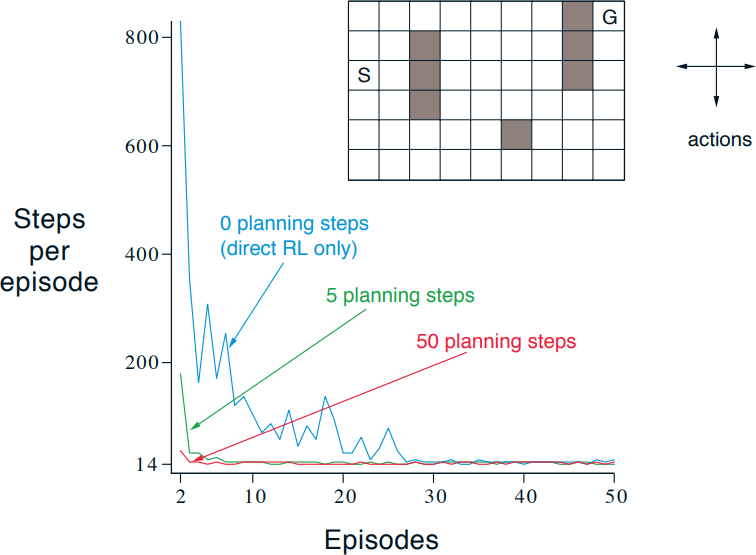
\includegraphics[width = 0.75 \textwidth]{4.44.png}
    \caption
    {
        A simple maze (inset) and the average learning curves for Dyna-Q agents varying in ther number of planning steps ($n$) per real step.
        The task is to travel from $\mathsf S$ to $\mathsf G$ as quickly as possible.
    }
    \label{fig:8.2}
\end{figure}

\end{exercise}

% -------------------------------------------------------------------------------- %

\begin{solution}

\phantom{}

\end{solution}

% -------------------------------------------------------------------------------- %
